\section{Diskussion}
\label{sec:Diskussion}
Die Evakuierungskurven der Pumpen (vgl. Abb. \ref{fig:drehEvac} und \ref{fig:turboEvac}) sind gewissermaßen erfolgreich gelungen.
Bei der Drehschieberpumpe ist eine hervorragende Einteilung der gewünschten 3 Bereiche möglich.
Lediglich waren bei der Turbomolekularpumpe die Messintervalle zu groß und die Bereiche des konstanten logarithmischen Ausdruckes leideten darunter.
Somit war eine Berechnung der Saugvermögen im Entfernten des Enddruckes nur wage möglich.

Bei den Leckratenmessungen hingegen klappte es beide Male für alle Gleichgewichtsdrücke den linearen Druckanstieg deutlich zu machen 
(vgl. Abb. \ref{fig:drehLeck05} bis \ref{fig:drehLeck100} und \ref{fig:turboLeck2} bis \ref{fig:turboLeck5}).

In \autoref{fig:dreh} sind die verschiedenen Saugvermögen der einzelnen Methoden und Messreihen der Drehschieberpumpe aufgeführt,
in \autoref{fig:turbo} die der Turbomolekularpumpe. Bei der Drehschieberpumpe bietet sich aufgrund der großen Unterschiede der Druckbereiche
ein halblogarithmischer Plot an.

Die Herstellerangaben der Pumpen sind $\qty{77}{\liter\per\second}$ für die Turbomolekularpumpe und $1.28$ bis $1.53 \unit{\liter\per\second}$ für die Drehschieberpumpe.
Hierbei ist wohl am deutlichsten zu erkennen, dass vor allem die Messung der Turbomolekularpumpe eine deutliche Abweichung dieser hervorweist.
Dahingegen kann zumindest der Wert $S_{L,10}$ der Drehschieberpumpe den Hersteller in seinem Fehler bestätigen. Ob aber dadurch von einem Erfolg der Messreihe zu sprechen ist, ist fraglich.
Es fällt jedoch auf, dass sich trotz dieser deutlichen Differenzen mehrfach die Methoden der Evakuierungskurve und der Leckratenmessung in ihren Fehlern überschneiden.

Es muss natürlich in Anbetracht gezogen werden, dass lediglich das effektive Saugvermögen
\begin{equation*}
    S_{eff} = \frac{S_0\cdot L}{S_0 + L}
\end{equation*}
mit dem Leitwert $L$ der Rohre und dem theoretischen Saugvermögen $S_0$ bestimmt werden kann.
Der Hersteller ist natürlich unter professionellen Laborbedingungen daran interessiert mit einer höchstmöglichen Saugleistung sein Produkt zu bewerben.
Von daher werden sicherlich maßgefertigte Anpassungen an der Messvorrichtung vorgenommen um beispielsweise genannte Leitwerte zu minimieren und
der ausgewählten Pumpe eine möglichst ideale Umgebung zu schaffen.
\begin{figure}
    \centering
    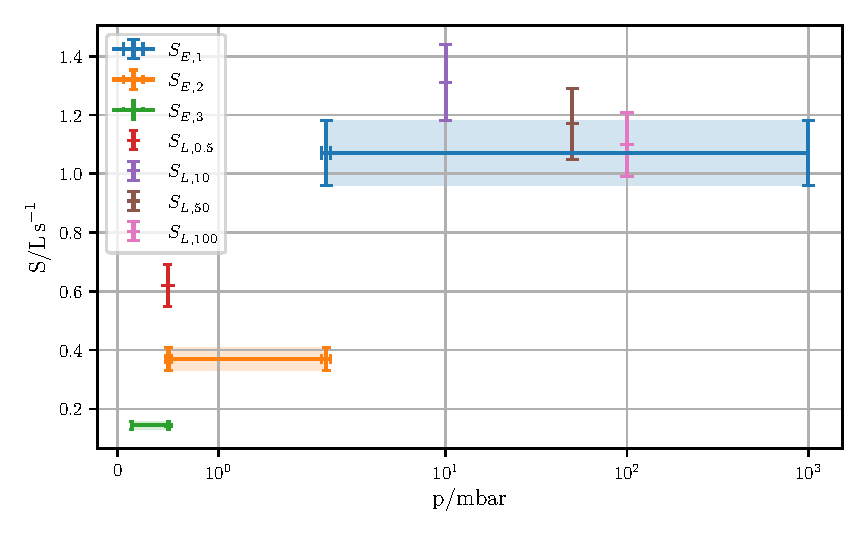
\includegraphics[width=0.8\textwidth]{abb/plot1.pdf}
    \caption{Die Saugvermögen der verschiedenen Messreihen zur Drehschieberpumpe}
    \label{fig:dreh}
\end{figure}
\begin{figure}
    \centering
    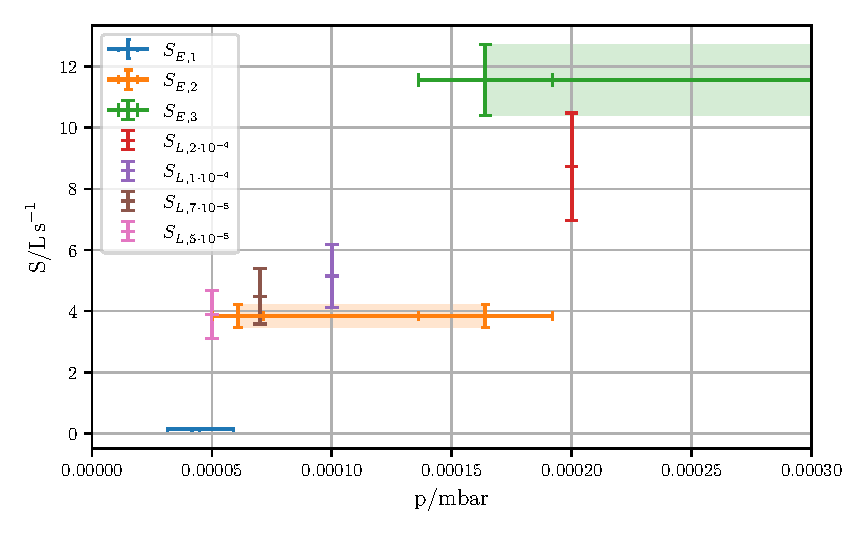
\includegraphics[width=0.8\textwidth]{abb/plot2.pdf}
    \caption{Die Saugvermögen der verschiedenen Messreihen zur Turbomolekularpumpe}
    \label{fig:turbo}
\end{figure}

\newpage

\begin{figure}
    \centering
    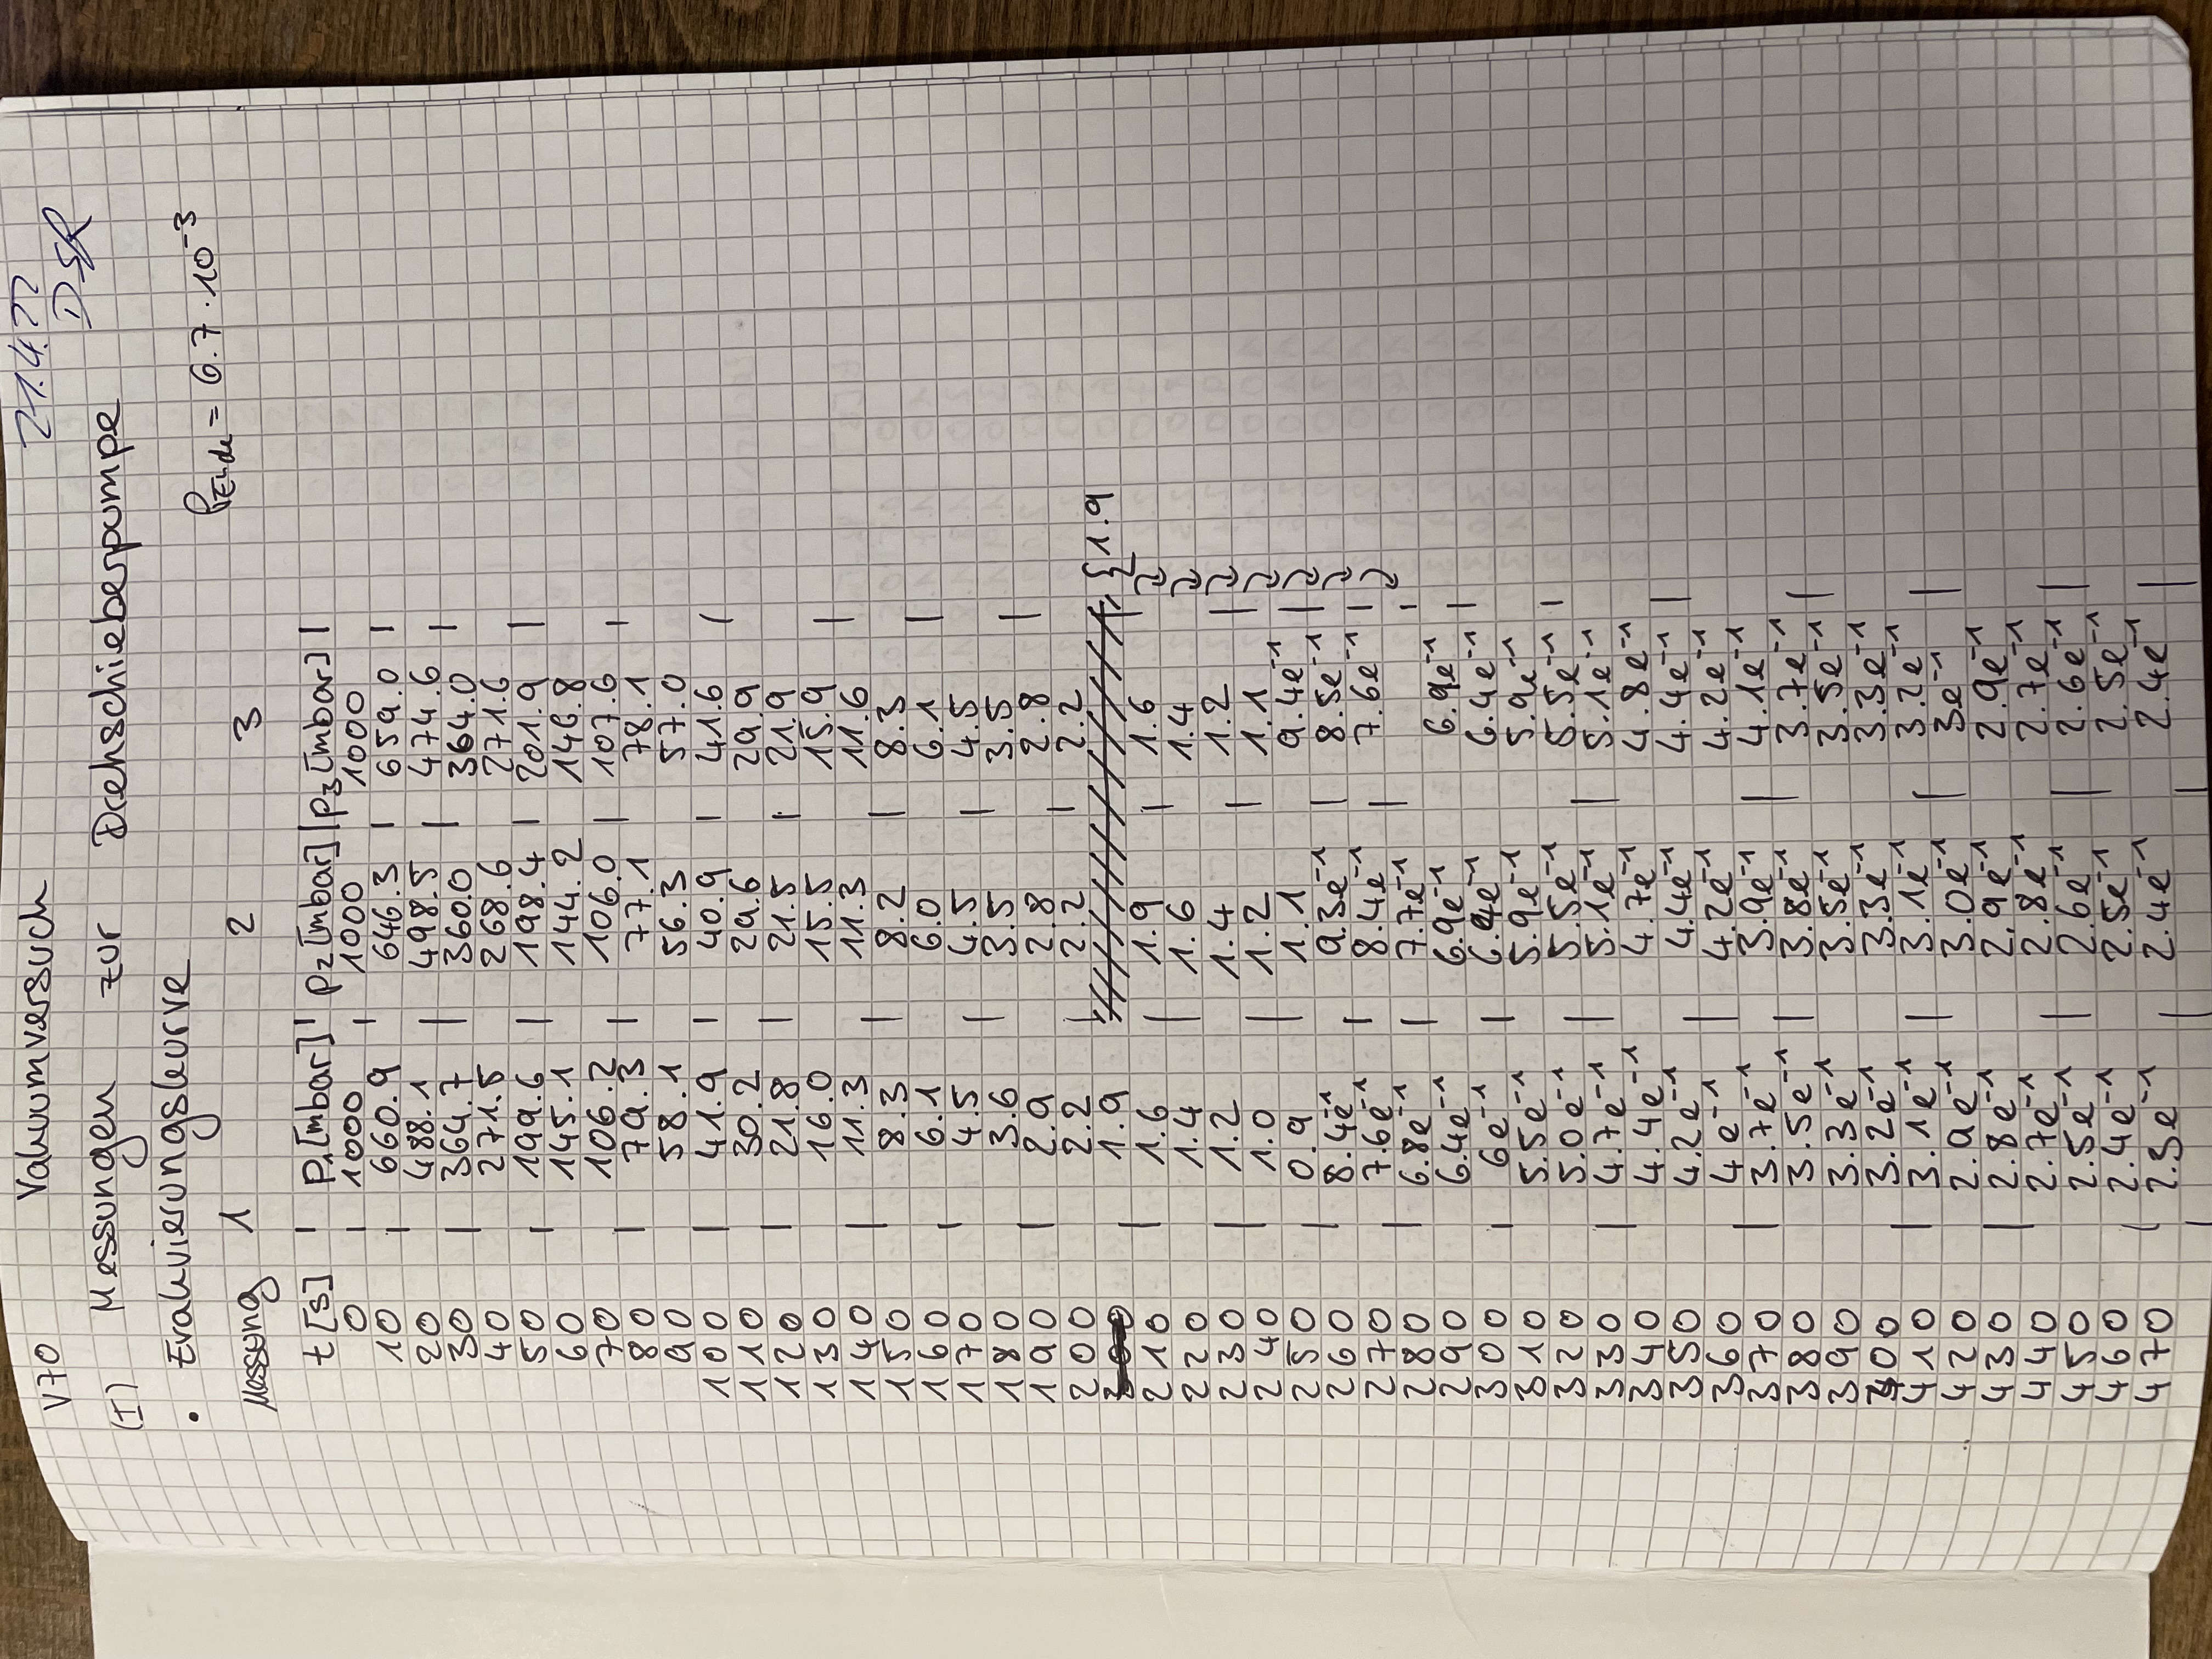
\includegraphics[width=0.7\textwidth]{abb/IMG_3226.jpg}
\end{figure}
\begin{figure}
    \centering
    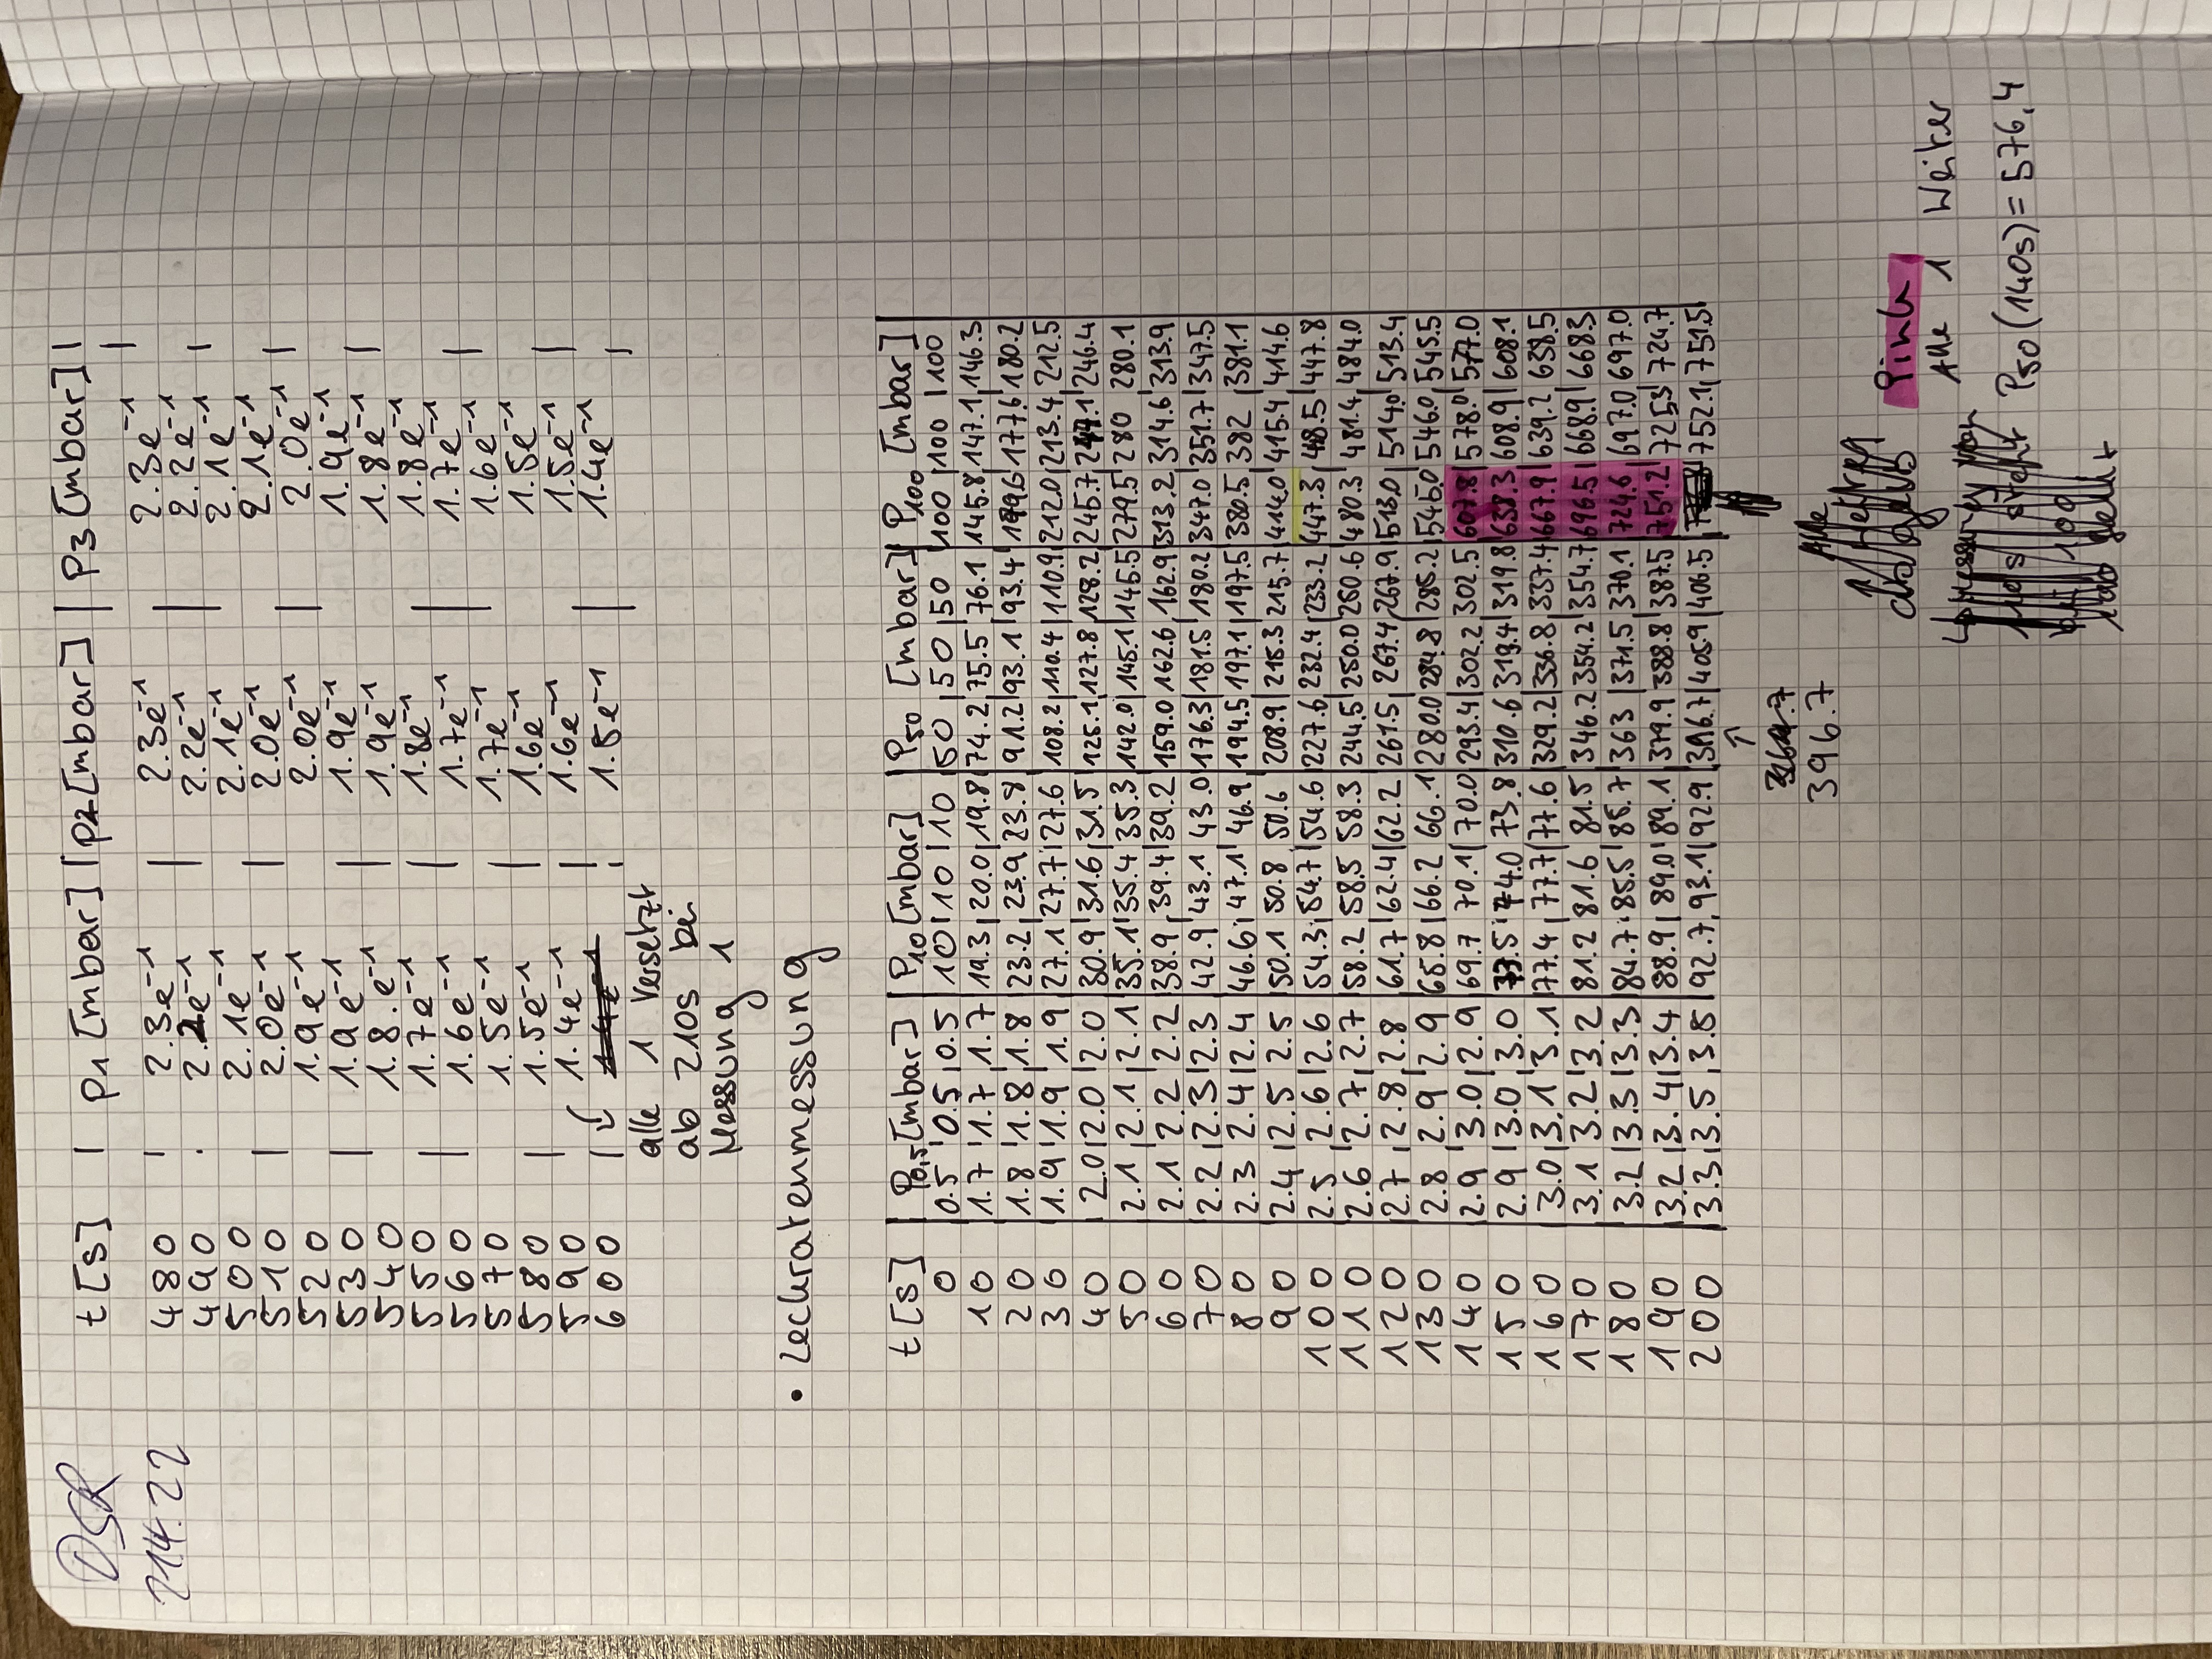
\includegraphics[width=0.7\textwidth]{abb/IMG_3227.jpg}
\end{figure}
\begin{figure}
    \centering
    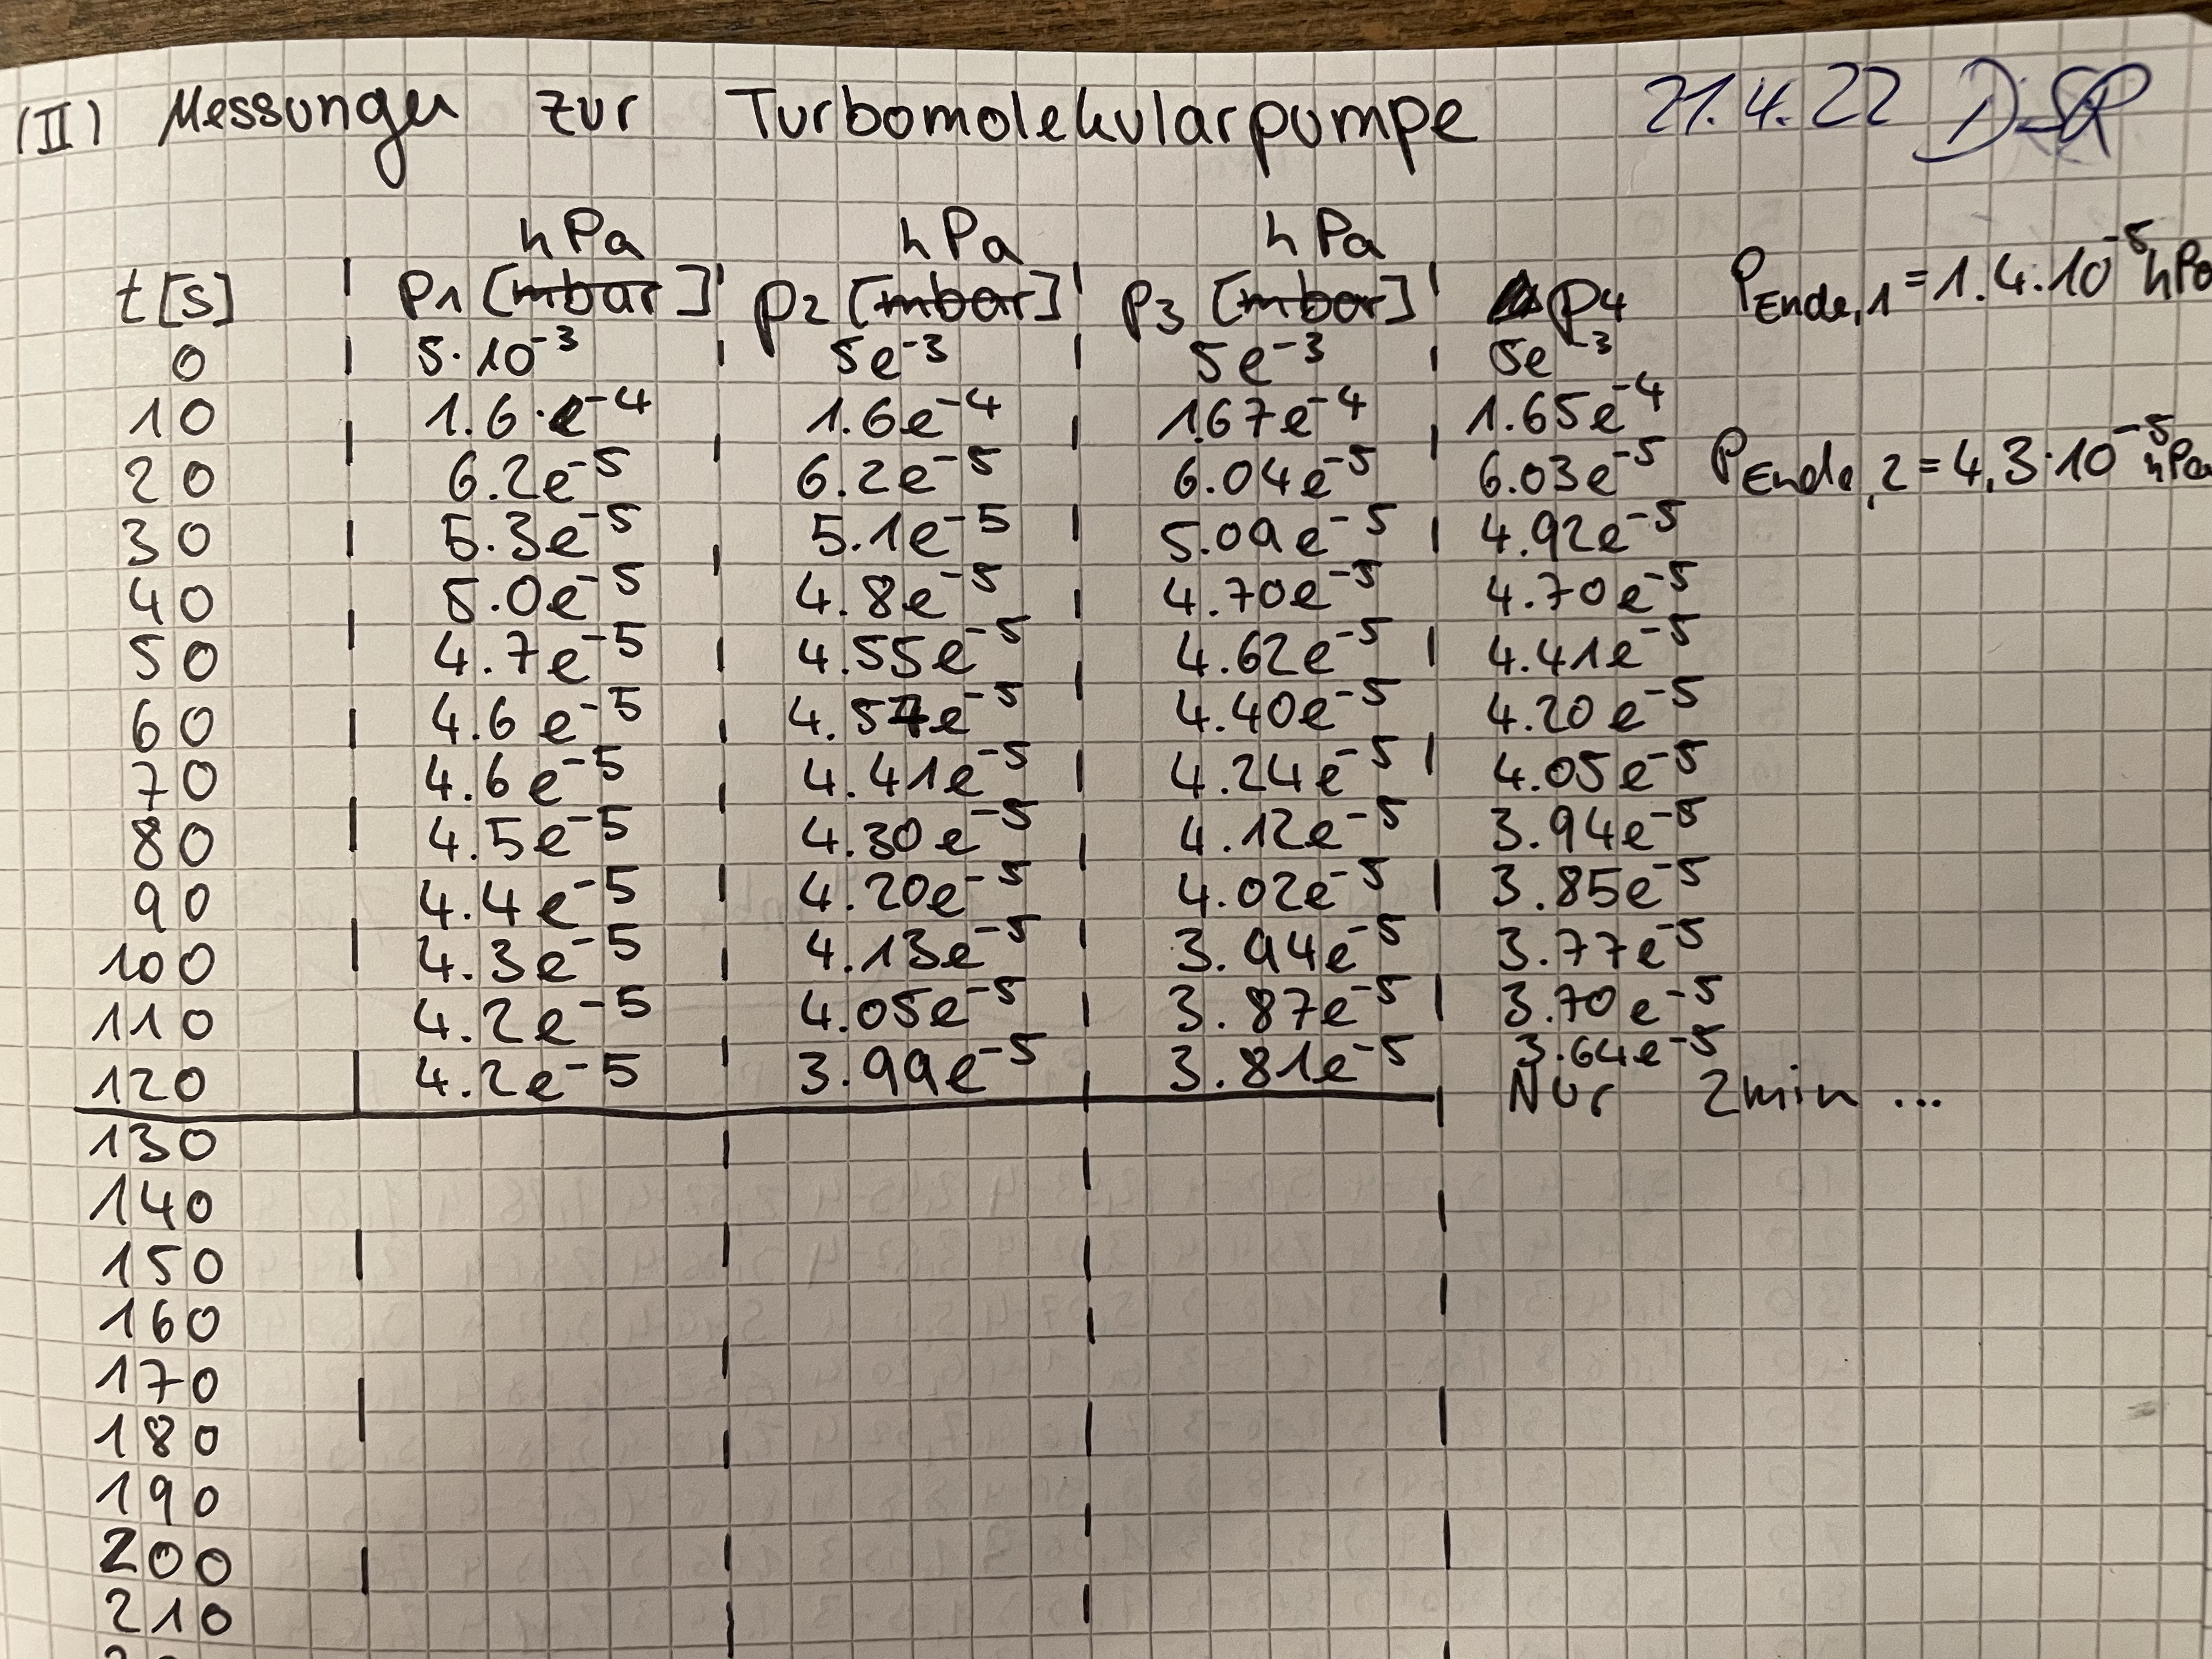
\includegraphics[width=0.7\textwidth]{abb/IMG_3228.jpg}
\end{figure}
\begin{figure}
    \centering
    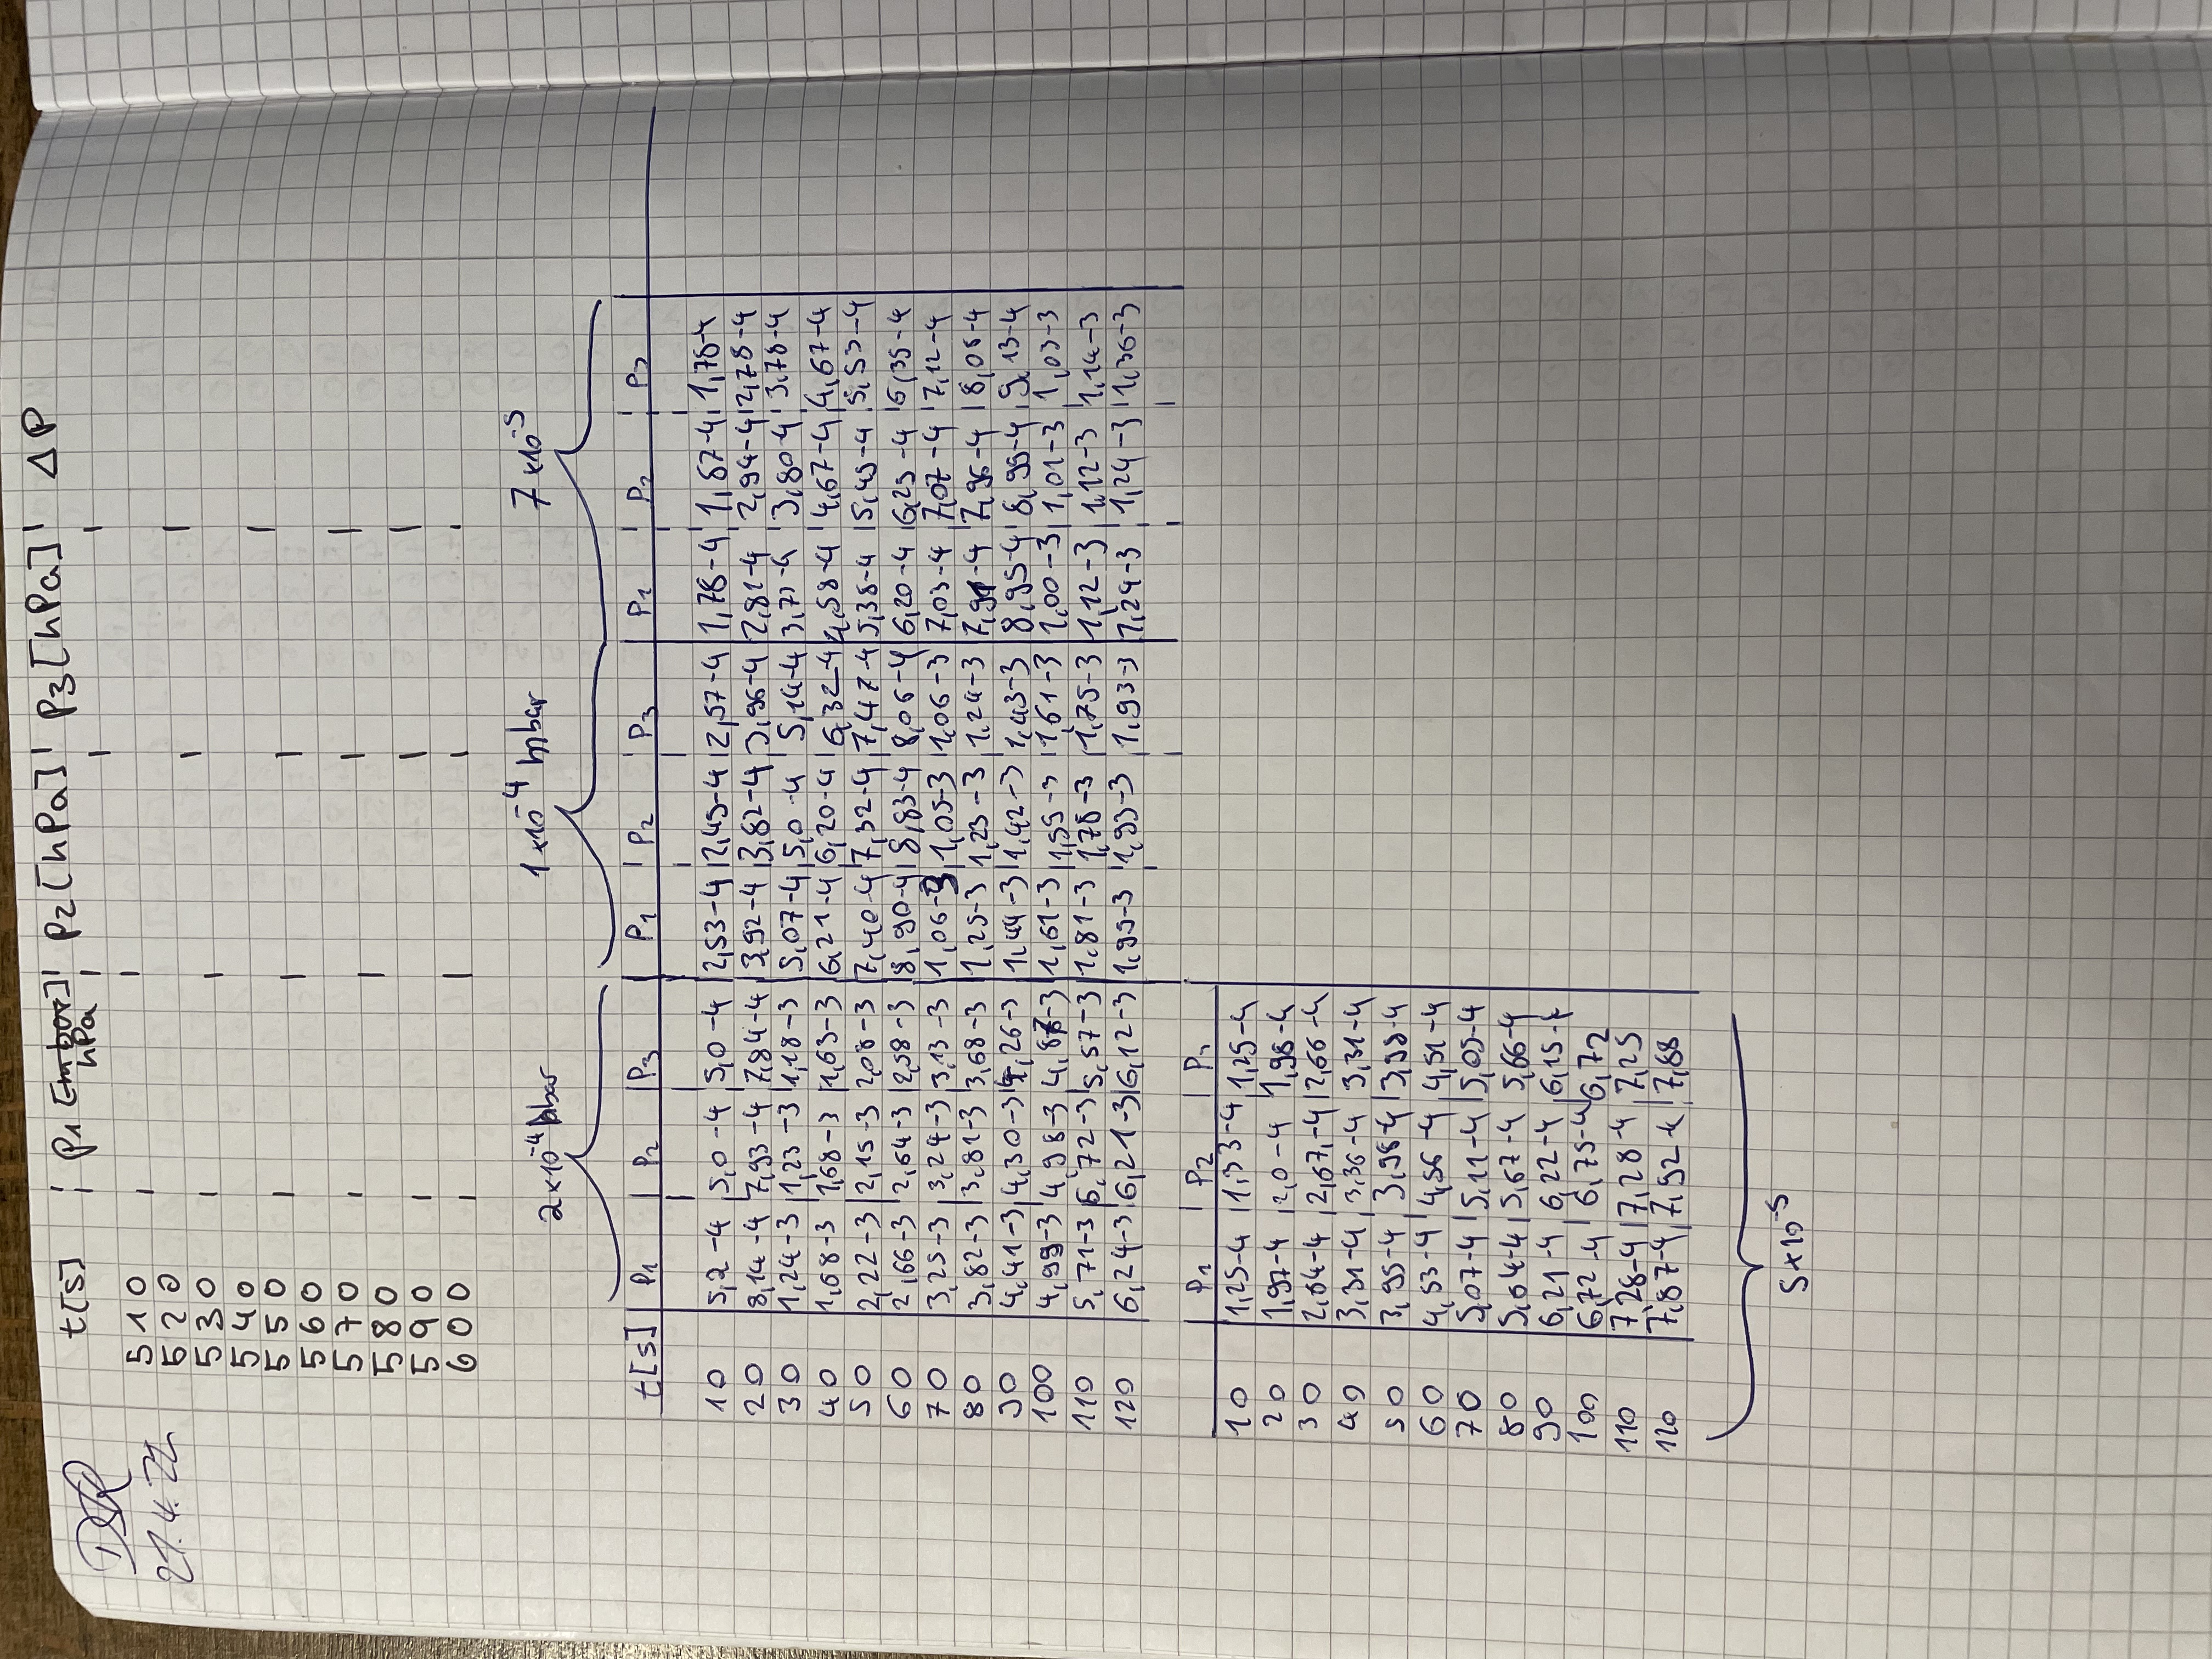
\includegraphics[width=0.7\textwidth]{abb/IMG_3229.jpg}
\end{figure}